\documentclass[11pt, oneside]{article}   	% use "amsart" instead of "article" for AMSLaTeX format
\usepackage{geometry}                		% See geometry.pdf to learn the layout options. There are lots.
\geometry{a4paper}                   		% ... or a4paper or a5paper or ... 

\usepackage{amssymb}
\usepackage{amsmath}
\usepackage{tikz}
\usetikzlibrary{trees}

\tikzstyle{decision} = [circle,draw,text width=1em, text centered]
\tikzstyle{payoff} = [circle, minimum width=0.5em,fill]
\tikzstyle{level 1}=[level distance=2.5cm, sibling distance=6cm]
\tikzstyle{level 2}=[level distance=2.5cm, sibling distance=3cm]
\tikzstyle{level 3}=[level distance=2.5cm, sibling distance=1.5cm]

\title{Decision Tree for a Signalling Game}
\author{Nick Cao}

\begin{document}
\maketitle

The extensive form of the signalling game is as follows:
\vskip 2em
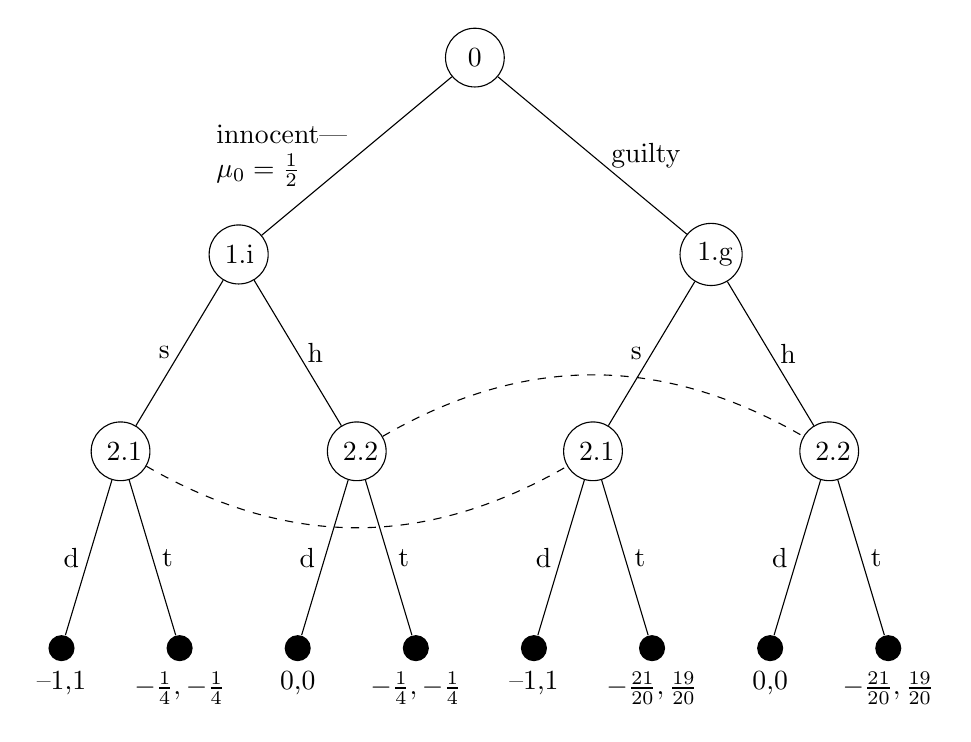
\begin{tikzpicture}
%\draw[help lines] (-5,-8) grid (5,0);
\node[decision] {0}
	child{ node[decision] {1.i}
		child{ node[decision] (2x3) {2.1}
    		child{ node[payoff, label=below: {--1,1}] {}
    			edge from parent
    			node[left] {d}
			}
			child{ node[payoff, label=below: {$-\frac{1}{4},-\frac{1}{4}$}] {}
    			edge from parent
    			node[right] {t}
			}
			edge from parent
			node[left]{s}
		}
		child{ node[decision] (2x1) {2.2}
			child{ node[payoff, label=below: {0,0}] {}
				edge from parent
				node[left] {d}
			}
			child{ node[payoff, label=below: {$-\frac{1}{4},-\frac{1}{4}$}] {}
				edge from parent
				node[right] {t}
			}
			edge from parent
			node[right] {h}
		}
		edge from parent
		node[left, align=left] {innocent--- \\ $\mu_0=\frac{1}{2}$}
	} 
	child{ node[decision] {1.g}
		child{ node[decision] (2x4) {2.1}
    		child{ node[payoff, label=below: {--1,1}] {}
    			edge from parent
    			node[left] {d}
    		}
    		child{ node[payoff, label=below: {$-\frac{21}{20},\frac{19}{20}$}] {}
        			edge from parent
        			node[right] {t}
        		}
			edge from parent
			node[left] {s}
		}
		child{ node[decision] (2x2) {2.2}
			child{ node[payoff, label=below: {0,0}] {}
				edge from parent
				node[left] {d}
			}
			child{ node[payoff, label=below: {$-\frac{21}{20},\frac{19}{20}$}] {}
				edge from parent
				node[right] {t}
			}
			edge from parent
			node[right] {h}
		}	
	edge from parent
	node[right] {\ guilty}
	}
	;
	\draw[dashed] (2x1) to [out=30,in=150]  (2x2) ;
	\draw[dashed] (2x3) to [out=330,in=210]  (2x4) ;
\end{tikzpicture}

\end{document}